%%%%%%%%%%%%%%%%%%%%%%%%%%%%%%%%%%%%%%%%%%%%%%%%%%%%%%%%%%%%
%% This Beamer template was created by Cameron Bracken.
%% Anyone can freely use or modify it for any purpose
%% without attribution.
%%
%% Last Modified: January 9, 2009
%%

\documentclass[xcolor=x11names,compress]{beamer}

%% General document %%%%%%%%%%%%%%%%%%%%%%%%%%%%%%%%%%
\usepackage[numberedbib]{apacite}
\usepackage{graphicx}
\usepackage{wrapfig}
\usepackage{enumerate}
\usepackage{subfig}
\usepackage{tikz}
\usepackage{fancybox}
\usepackage{coqdoc}
\usepackage{amsmath,amssymb}
\usetikzlibrary{decorations.fractals}
%%%%%%%%%%%%%%%%%%%%%%%%%%%%%%%%%%%%%%%%%%%%%%%%%%%%%%
%% Beamer Layout %%%%%%%%%%%%%%%%%%%%%%%%%%%%%%%%%%
\useoutertheme[subsection=false,shadow]{miniframes}
\useinnertheme{default}
\usefonttheme{serif}
%\usepackage{palatino}

%\setbeamerfont{title like}{shape=\scshape}
%\setbeamerfont{frametitle}{shape=\scshape}

\setbeamercolor*{lower separation line head}{bg=DeepSkyBlue4}
\setbeamercolor*{normal text}{fg=black,bg=white}
\setbeamercolor*{alerted text}{fg=red}
\setbeamercolor*{example text}{fg=black}
\setbeamercolor*{structure}{fg=black}

\setbeamercolor*{palette tertiary}{fg=black,bg=black!10}
\setbeamercolor*{palette quaternary}{fg=black,bg=black!10}

\renewcommand{\(}{\begin{columns}}
\renewcommand{\)}{\end{columns}}
\newcommand{\<}[1]{\begin{column}{#1}}
\renewcommand{\>}{\end{column}}

%%%%%%%%%%%%%%%%%%%%%%%%%%%%%%%%%%%%%%%%%%%%%%%%%%



\begin{document}


%%%%%%%%%%%%%%%%%%%%%%%%%%%%%%%%%%%%%%%%%%%%%%%%%%%%%%
%%%%%%%%%%%%%%%%%%%%%%%%%%%%%%%%%%%%%%%%%%%%%%%%%%%%%%
%\section{\scshape Introduction}
\begin{frame}
\title{An Artificial Science for System Value Engineering and Assurance}
%\subtitle{SUBTITLE}
\author{
Chong Tang,  Kevin Sullivan, Ke Dou, Koleman Nix\\
{\it Department of Computer Science}\\
{\it University of Virginia}
}
\date{

\includegraphics[scale=0.2]{figures/logo2}

\today
}
\titlepage
\end{frame}

%%%%%%%%%%%%%%%%%%%%%%%%%%%%%%%%%%%%%%%%%%%%%%%%%%%%%%
%%%%%%%%%%%%%%%%%%%%%%%%%%%%%%%%%%%%%%%%%%%%%%%%%%%%%%
%\begin{frame}{Outline}
%\tableofcontents
%\end{frame}

%%%%%%%%%%%%%%%%%%%%%%%%%%%%%%%%%%%%%%%%%%%%%%%%%%%%%%
%%%%%%%%%%%%%%%%%%%%%%%%%%%%%%%%%%%%%%%%%%%%%%%%%%%%%%
\section{\scshape Introduction}
\subsection{Problems}
\begin{frame}{Problems}
\framesubtitle{Weak engineering foundations}
\begin{itemize}
\item Weak understanding of system qualities
\item Weak ability to engineer system qualities
\item Poor understanding of relationships among qualities
\item Lacking frameworks for reasoning about tradeoffs
\item Weak ability to manage  qualities across lifecycle
\end{itemize}
\vspace{0.5cm}
These engineering problems are in turn rooted in weak science.
\end{frame}

%%%%%%%%%%%%%%%%%%%%%%%%%%%%%%%%%%%%%%%%%%%%%%%%%%%%%%
%%%%%%%%%%%%%%%%%%%%%%%%%%%%%%%%%%%%%%%%%%%%%%%%%%%%%%
\begin{frame}{Problems}
\framesubtitle{Weak scientific foundations}
\begin{itemize}
\item Research has often been informal and imprecise
\item Theories expressed in natural language, tables, graphics
\item No use of math, computational, and logical notations
\end{itemize}
\vspace{0.5cm}
Consequently we also lack foundations for automated tools for assisting with such issues.
\end{frame}

%%%%%%%%%%%%%%%%%%%%%%%%%%%%%%%%%%%%%%%%%%%%%%%%%%%%%%
%%%%%%%%%%%%%%%%%%%%%%%%%%%%%%%%%%%%%%%%%%%%%%%%%%%%%%
\subsection{Purpose}
\begin{frame}{Purpose}
To provide a framework for:
\begin{itemize}
\item Communicating, reasoning about system qualities
\item Reasoning about tradeoffs among system qualities
\item Building formal languages to exress qualities
\item Formalizing theories with formal notations
\item Providing automated tools to assist with the above
\end{itemize}
\end{frame}

%%%%%%%%%%%%%%%%%%%%%%%%%%%%%%%%%%%%%%%%%%%%%%%%%%%%%%
%%%%%%%%%%%%%%%%%%%%%%%%%%%%%%%%%%%%%%%%%%%%%%%%%%%%%%
\section{State of The Art}
\subsection{Ross}
\begin{frame}{State of The Art}
\framesubtitle{Ross's Semantic Approach \cite{Ross:changeability}}
\begin{itemize}
\item \textbf{Problem:}\\No precise understanding of particular system properties
\item \textbf{Key Idea:} \\A semantic approach for defining change-related ility terms
\item \textbf{Main Contributions:}
\begin{itemize}
\item {\em Informal grammar} for changeability requirements
\item Rules for {\em classifying statements} by {\em ility}
\item Providing {\em semantics} to ility terms
\end{itemize}
\end{itemize}
\end{frame}

%%%%%%%%%%%%%%%%%%%%%%%%%%%%%%%%%%%%%%%%%%%%%%%%%%%%%%
%%%%%%%%%%%%%%%%%%%%%%%%%%%%%%%%%%%%%%%%%%%%%%%%%%%%%%

\begin{frame}{Ross's semantic basis approach \footnote{Figures from \cite{Ross:changeability}}}
\begin{figure}
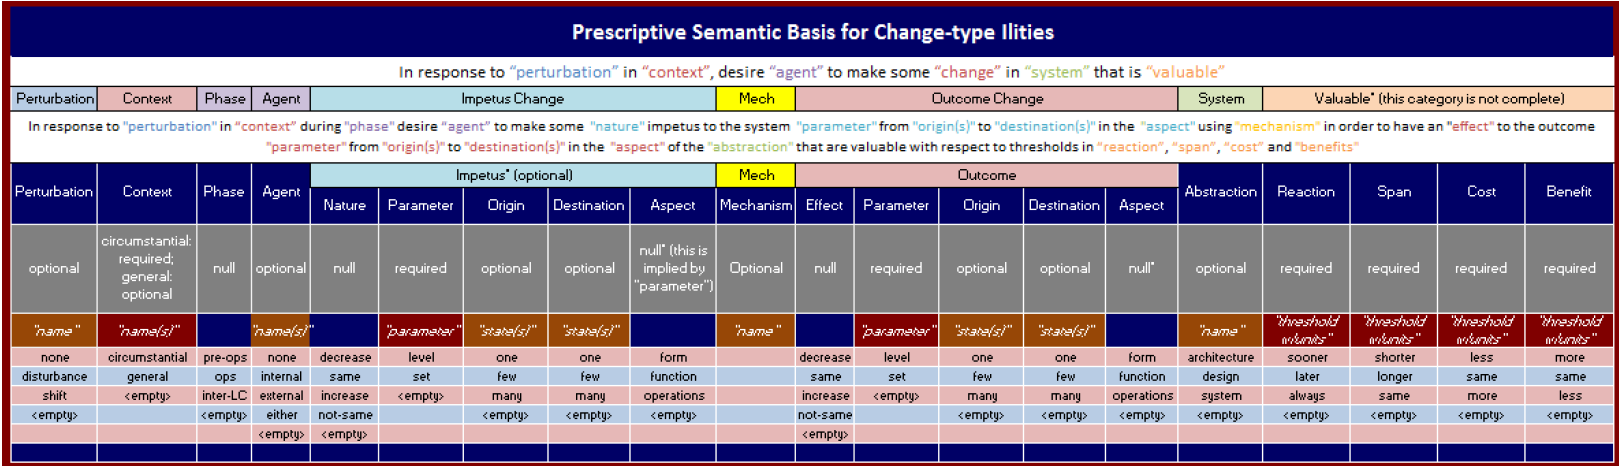
\includegraphics[scale=0.22]{figures/semantic}
%\caption{}
%\end{figure}
\vspace{0.4cm}
%\begin{figure}
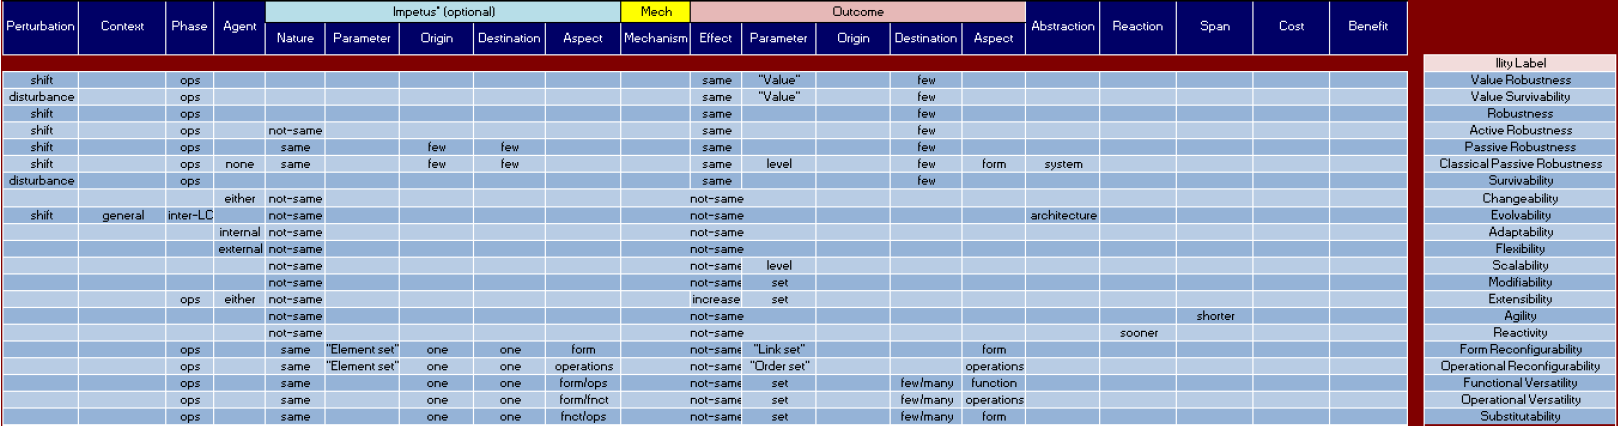
\includegraphics[scale=0.22]{figures/usesemantic}
\caption{Ross's prescriptive semantic basis for change-type ilites}
\end{figure}
\end{frame}


%%%%%%%%%%%%%%%%%%%%%%%%%%%%%%%%%%%%%%%%%%%%%%%%%%%%%%
%%%%%%%%%%%%%%%%%%%%%%%%%%%%%%%%%%%%%%%%%%%%%%%%%%%%%%

\begin{frame}{Ross's semantic basis approach}
\begin{itemize}
\item \textbf{Pros:} \\
	Defining change-related ilities requirements statements
\item \textbf{Cons:} \\
	Informal, not computable, hard to evaluate and evolve
\end{itemize}
\end{frame}

%%%%%%%%%%%%%%%%%%%%%%%%%%%%%%%%%%%%%%%%%%%%%%%%%%%%%%
%%%%%%%%%%%%%%%%%%%%%%%%%%%%%%%%%%%%%%%%%%%%%%%%%%%%%%
\subsection{Boehm}
\begin{frame}{State of The Art}
\framesubtitle{Boehm's top-down Taxonomy \cite{Boehm:ontology}}
\begin{itemize}
\item \textbf{Problem:}\\System designs are deficient in balancing system ilites
\item \textbf{Key Ideas:}
	\begin{itemize}
	\item Defining language grammer for full range of ilities
	\item Balancing ility values for the system's stakeholders
	\end{itemize}
\item \textbf{Main Contributions:}
\begin{itemize}
\item Proposing a stakeholder-value based property hierarchy
\item An ontology for reasoning about a system's ilities
\item Studied Synergies and Conflicts among key properties
\end{itemize}
\end{itemize}
\end{frame}

%%%%%%%%%%%%%%%%%%%%%%%%%%%%%%%%%%%%%%%%%%%%%%%%%%%%%%
%%%%%%%%%%%%%%%%%%%%%%%%%%%%%%%%%%%%%%%%%%%%%%%%%%%%%%

\begin{frame}{Boehm's top-down Taxonomy \footnote{Figure from \cite{Boehm:ontology}}}
\begin{figure}
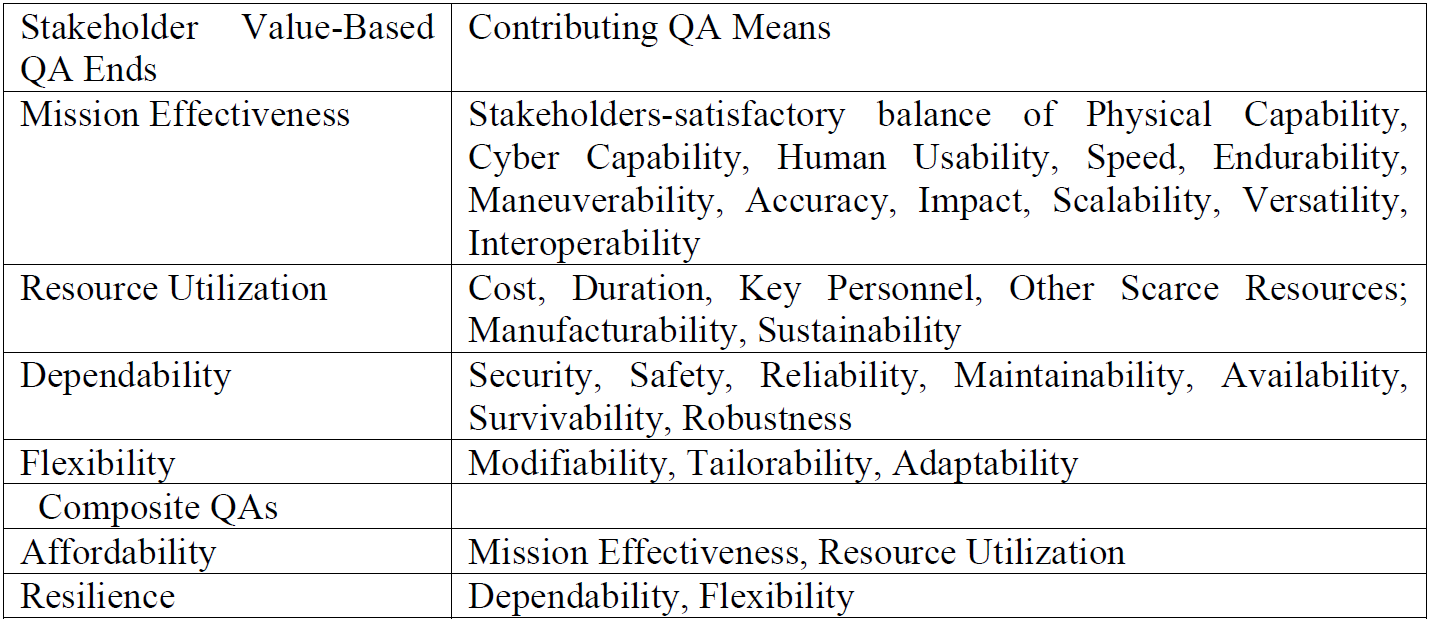
\includegraphics[scale=0.28]{figures/hierarchy}
\caption{Stakeholder-value based property means-ends hierarchy}
\end{figure}
\end{frame}

%%%%%%%%%%%%%%%%%%%%%%%%%%%%%%%%%%%%%%%%%%%%%%%%%%%%%%
%%%%%%%%%%%%%%%%%%%%%%%%%%%%%%%%%%%%%%%%%%%%%%%%%%%%%%

\begin{frame}{Boehm's top-down Taxonomy}
\begin{itemize}
\item \textbf{Pros:}
	\begin{itemize}
		\item Clarifying the nature of system ilities
		\item Reasoning about the tradeoffs among ilities
		\item Addressing stakeholder value conflicts
	\end{itemize}
\item \textbf{Cons:}\\
	Informal, difficult to validate, hard to apply
\end{itemize}
\end{frame}

%%%%%%%%%%%%%%%%%%%%%%%%%%%%%%%%%%%%%%%%%%%%%%%%%%%%%%
%%%%%%%%%%%%%%%%%%%%%%%%%%%%%%%%%%%%%%%%%%%%%%%%%%%%%%
\subsection{Assurance Cases}
\begin{frame}{State of The Art}
\framesubtitle{Assurance Cases}
\begin{itemize}
	\item Claim - Assertion about key requirements and properties
    \item Evidence
	    \begin{itemize}
    		\item Testing, Proofs, Process and people, Review and analyses
	    \end{itemize}
    \item Argument - How the evidences support the claims
    \begin{itemize}
    	\item Inference rules: deterministic, probabilistic, qualitative
    \end{itemize}
    \item Inductive reasoning
    	\begin{itemize}
       	\item Providing evidence, not proof that the claim is certain
      	\end{itemize}
\end{itemize}
%\end{itemize}
\end{frame}

%%%%%%%%%%%%%%%%%%%%%%%%%%%%%%%%%%%%%%%%%%%%%%%%%%%%%%
%%%%%%%%%%%%%%%%%%%%%%%%%%%%%%%%%%%%%%%%%%%%%%%%%%%%%%

\begin{frame}{Assurance Cases \footnote{Figure from \cite{Kelly:GSN}}}
\begin{figure}
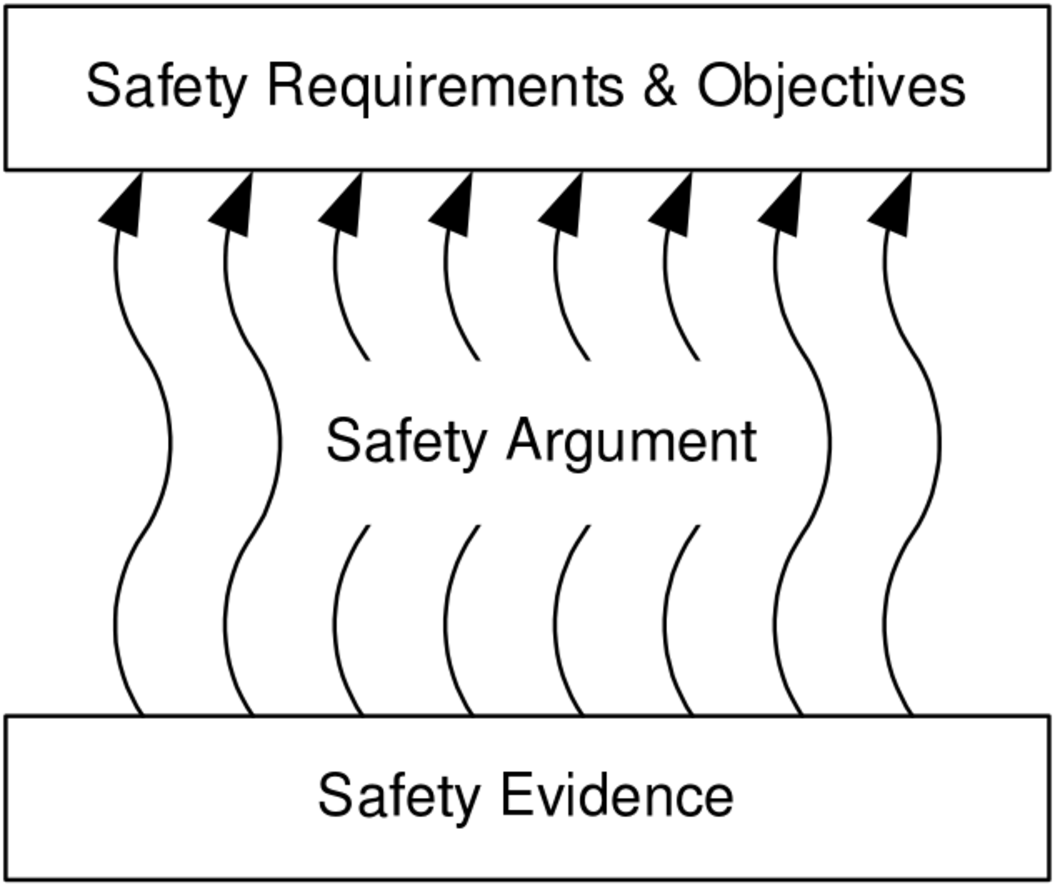
\includegraphics[scale=0.3]{figures/assurance-case}
\caption{The relationship among safety case elements}
\end{figure}
\end{frame}


%%%%%%%%%%%%%%%%%%%%%%%%%%%%%%%%%%%%%%%%%%%%%%%%%%%%%%
%%%%%%%%%%%%%%%%%%%%%%%%%%%%%%%%%%%%%%%%%%%%%%%%%%%%%%
\subsection{GSN}
\begin{frame}{State of The Art}
\framesubtitle{Kelly's Goal Structuring Notation \cite{Kelly:GSN}}
\begin{itemize}
\item \textbf{Problem:}\\Safety arguments are often poorly communicated
\item \textbf{Key Idea:} \\Develop safety cases in a reader-friendly manner
\item \textbf{Main Contributions:}
\begin{itemize}
    \item Using graphical notations to annotate the assurance cases
    \item Applying \emph{inductive} argumentation to safety cases
\end{itemize}
\end{itemize}
\end{frame}

%%%%%%%%%%%%%%%%%%%%%%%%%%%%%%%%%%%%%%%%%%%%%%%%%%%%%%
%%%%%%%%%%%%%%%%%%%%%%%%%%%%%%%%%%%%%%%%%%%%%%%%%%%%%%

\begin{frame}{Kelly's Goal Structuring Notation}
\begin{figure}
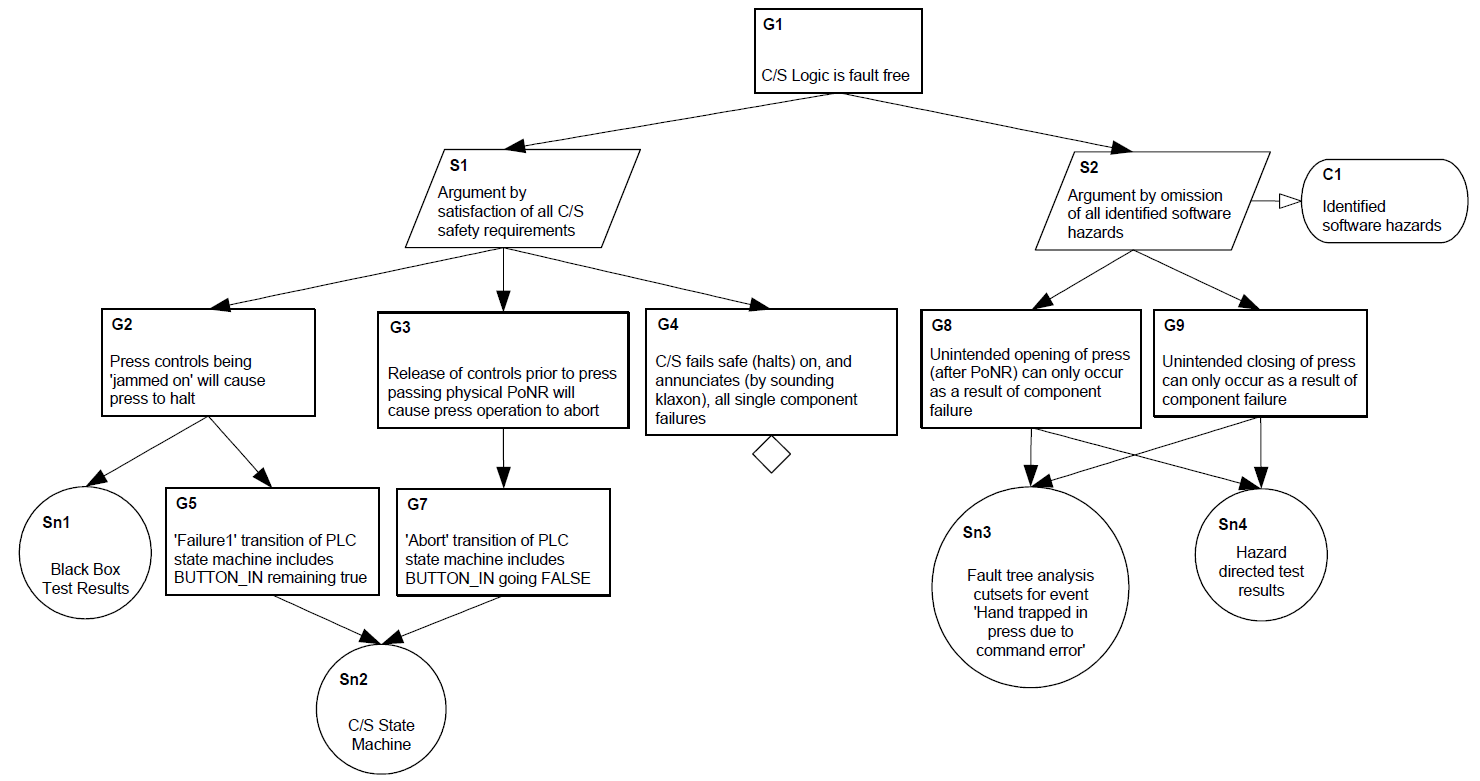
\includegraphics[scale=0.3]{figures/gsn}
\caption{Example GSN (Figure from \cite{Kelly:GSN})}
\end{figure}
\end{frame}

%%%%%%%%%%%%%%%%%%%%%%%%%%%%%%%%%%%%%%%%%%%%%%%%%%%%%%
%%%%%%%%%%%%%%%%%%%%%%%%%%%%%%%%%%%%%%%%%%%%%%%%%%%%%%

\begin{frame}{Kelly's GSN safety argument notation}
\begin{itemize}
\item \textbf{Pros:} \\
	Facilitate comprehension and communication of arguments
\item \textbf{Cons:} \\
	Informal, syntax rules are defined in prose text, not scale
\end{itemize}
\end{frame}

%%%%%%%%%%%%%%%%%%%%%%%%%%%%%%%%%%%%%%%%%%%%%%%%%%%%%%
%%%%%%%%%%%%%%%%%%%%%%%%%%%%%%%%%%%%%%%%%%%%%%%%%%%%%%
\subsection{Rushby}
\begin{frame}{State of The Art}
\framesubtitle{Rushby's Theory \cite{Rushby:formalism}}
\begin{itemize}
\item \textbf{Problem:}\\Increasing confidence in the soundness of a given case
\item \textbf{Key Ideas:}
			\begin{itemize}
			\item Applying formalism to safety cases
			\item Eliminating logic doubt and focusing on epistemic logic
			\end{itemize}
\item \textbf{Main Contributions:}
\begin{itemize}
	\item Formalizing parts of a safety argument into deductive logic
	\item Providing mechnized support for assurance case argument
	\item Helping engineers focus on evidence instead of argument
\end{itemize}
\end{itemize}
\end{frame}

%%%%%%%%%%%%%%%%%%%%%%%%%%%%%%%%%%%%%%%%%%%%%%%%%%%%%%
%%%%%%%%%%%%%%%%%%%%%%%%%%%%%%%%%%%%%%%%%%%%%%%%%%%%%%
\begin{frame}{Rushby's Theory}
\begin{itemize}
\item \textbf{Pros:} \\
	Improving efficiency and cost of safety argument checking
\item \textbf{Cons:} \\
	No empirical evidence
\end{itemize}
\end{frame}

%%%%%%%%%%%%%%%%%%%%%%%%%%%%%%%%%%%%%%%%%%%%%%%%%%%%%%
%%%%%%%%%%%%%%%%%%%%%%%%%%%%%%%%%%%%%%%%%%%%%%%%%%%%%%

\subsection{Knight}
\begin{frame}{State of The Art}
\framesubtitle{Knight's Assurance Based Development \cite{Knight:Assurance}}
\begin{itemize}
\item \textbf{Problem:}\\Assurance cases often fail to guide developers' decisions
\item \textbf{Key Idea:} \\Co-developing the software system and its assurance case
\item \textbf{Main Contributions:}
\begin{itemize}
	\item Integrating assurance into development process.
    \item Assurance requirements drive development decisions
\end{itemize}
\end{itemize}

\end{frame}

%%%%%%%%%%%%%%%%%%%%%%%%%%%%%%%%%%%%%%%%%%%%%%%%%%%%%%
%%%%%%%%%%%%%%%%%%%%%%%%%%%%%%%%%%%%%%%%%%%%%%%%%%%%%%
\begin{frame}{Knight's Assurance Based Development}
\begin{itemize}
\item \textbf{Pros:} \\
	Detecting the assurance difficulties from the earliest stages
\item \textbf{Cons:} \\
	Hard to validate that their approach is optimal
\end{itemize}
\end{frame}

%%%%%%%%%%%%%%%%%%%%%%%%%%%%%%%%%%%%%%%%%%%%%%%%%%%%%%
%%%%%%%%%%%%%%%%%%%%%%%%%%%%%%%%%%%%%%%%%%%%%%%%%%%%%%

\subsection{Basir}
\begin{frame}{State of The Art}
\framesubtitle{Basir's Automatically Generated Argument \cite{Basir:safety}}
\begin{itemize}
\item \textbf{Problem:}\\Formal proofs are complex and machine-oriented
\item \textbf{Key Idea:} \\Automatically generating a safety argument by converting natural deduction style proofs
\item \textbf{Main Contributions:}
\begin{itemize}
	\item helps human understand the formal proofs
\end{itemize}
\end{itemize}

\end{frame}


%%%%%%%%%%%%%%%%%%%%%%%%%%%%%%%%%%%%%%%%%%%%%%%%%%%%%%
%%%%%%%%%%%%%%%%%%%%%%%%%%%%%%%%%%%%%%%%%%%%%%%%%%%%%%
\begin{frame}{Basir's Automatically Generated Argument}
\begin{itemize}
\item \textbf{Pros:} \\
	Providing easier-to-understand proofs
\item \textbf{Cons:} \\
    \begin{itemize}
	\item No benefit over an hand-generated, informal argument
    \item Far from satisfactory as the proofs contain too many details
    \end{itemize}
\end{itemize}
\end{frame}

%%%%%%%%%%%%%%%%%%%%%%%%%%%%%%%%%%%%%%%%%%%%%%%%%%%%%%
%%%%%%%%%%%%%%%%%%%%%%%%%%%%%%%%%%%%%%%%%%%%%%%%%%%%%%

\subsection{Bosch}
\begin{frame}{State of The Art}
\framesubtitle{Bosch's Mobile Service Oriented Architectures \cite{vanGurp:MOSOA}}
\begin{itemize}
\item \textbf{Problem:}\\It's hard to achieve success in realizing mobile services
\item \textbf{Key Idea:} \\Defining the architecture drivers that make success
\item \textbf{Main Contributions:}
\begin{itemize}
	\item Identified the goals for mobile service oriented architectures
	\item Identified ilities that influence the success of mobile services
	\item Predicted future trends of mobile service
\end{itemize}
\end{itemize}

\end{frame}


%%%%%%%%%%%%%%%%%%%%%%%%%%%%%%%%%%%%%%%%%%%%%%%%%%%%%%
%%%%%%%%%%%%%%%%%%%%%%%%%%%%%%%%%%%%%%%%%%%%%%%%%%%%%%

\subsection{Lundberg}
\begin{frame}{State of The Art}
\framesubtitle{Lundberg's Architecture Design Guidelines \cite{Lundberg:qualityattributes}}
\begin{itemize}
\item \textbf{Problem:}\\There are conflicts between modifiability and performance
\item \textbf{Key Idea:} \\Providing guidelines in software architecture design
\item \textbf{Main Contributions:}
\begin{itemize}
	\item A taxonomy for performance and modifiability related QA
	\item Four software architecture design evaluation approaches
	\item Four architecture design transformation strategies
	\item Eight guidelines in software architecture design

\end{itemize}
\end{itemize}

\end{frame}


%%%%%%%%%%%%%%%%%%%%%%%%%%%%%%%%%%%%%%%%%%%%%%%%%%%%%%
%%%%%%%%%%%%%%%%%%%%%%%%%%%%%%%%%%%%%%%%%%%%%%%%%%%%%%
\begin{frame}{Lundberg's Architecture Design Guidelines}
\begin{itemize}
\item \textbf{Pros:} \\
	\begin{itemize}
	\item Revealed the relationships among architecture, quality attributes, and implementation
	\item The guidelines are extracted from real industry experience
    \end{itemize}
\item \textbf{Cons:} \\
    \begin{itemize}
	\item Only focus on performance and modifiability
	\item Such studies may not fit domains other than software design
    \end{itemize}
\end{itemize}
\end{frame}


%%%%%%%%%%%%%%%%%%%%%%%%%%%%%%%%%%%%%%%%%%%%%%%%%%%%%%
%%%%%%%%%%%%%%%%%%%%%%%%%%%%%%%%%%%%%%%%%%%%%%%%%%%%%%
\subsection{Knight}
\begin{frame}{State of The Art}
\framesubtitle{Knight's Success Arguments \cite{Graydon:successarguments}}
\begin{itemize}
\item \textbf{Problem:}\\Failure rate of software development efforts is high
\item \textbf{Key Idea:} \\Defining success argument to establish confidence
\item \textbf{Main Contributions:}
\begin{itemize}
	\item Structuring and documenting the argument
	\item Recording the argument and exposing it to examinations

\end{itemize}
\end{itemize}

\end{frame}


%%%%%%%%%%%%%%%%%%%%%%%%%%%%%%%%%%%%%%%%%%%%%%%%%%%%%%
%%%%%%%%%%%%%%%%%%%%%%%%%%%%%%%%%%%%%%%%%%%%%%%%%%%%%%
\begin{frame}{Knight's Success Arguments}
\begin{itemize}
\item \textbf{Pros:} \\
	\begin{itemize}
	\item Helps structure the reasoning and expose it to criticism
	\item Helps explain the evidence to the reviewers
    \end{itemize}
\item \textbf{Cons:} \\
    \begin{itemize}
	\item Informal, Hard to validate
    \end{itemize}
\end{itemize}
\end{frame}


%%%%%%%%%%%%%%%%%%%%%%%%%%%%%%%%%%%%%%%%%%%%%%%%%%%%%%
%%%%%%%%%%%%%%%%%%%%%%%%%%%%%%%%%%%%%%%%%%%%%%%%%%%%%%
\section{Approach}
\begin{frame}{Our approach}
\begin{itemize}
		\item Combining Bosch's innovation experiment systems  theory
        \item Integrating Boehm's theory and Ross's approach
		\item Using rigorous formal specification and software synthesis
		\item Refining and expressing quality theories using Coq
		\item Building web-based tools to implement the theory concepts
		\item Driving theory testing, evolution, and validation with tools
\end{itemize}
\end{frame}

%%%%%%%%%%%%%%%%%%%%%%%%%%%%%%%%%%%%%%%%%%%%%%%%%%%%%%
%%%%%%%%%%%%%%%%%%%%%%%%%%%%%%%%%%%%%%%%%%%%%%%%%%%%%%
\begin{frame}{Framework Architecture}
\begin{figure}
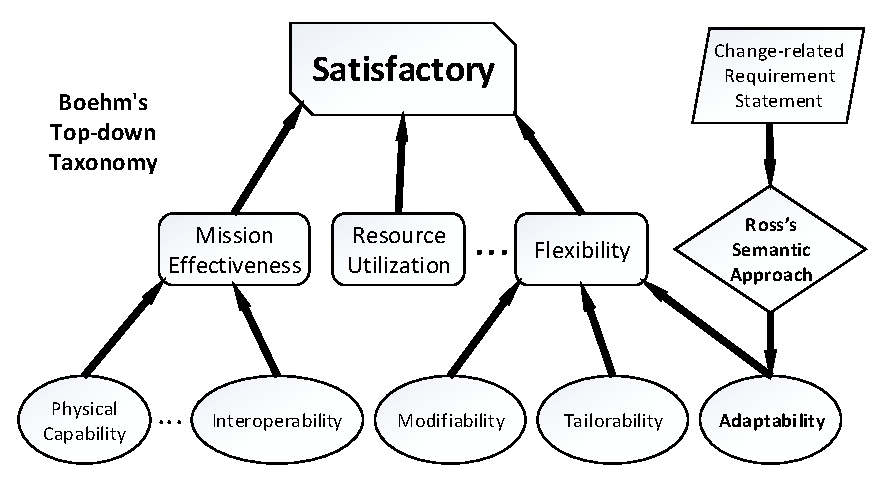
\includegraphics[scale=0.6]{figures/architecture}
\caption{The overall architecture of our framework}
\end{figure}
\end{frame}

%%%%%%%%%%%%%%%%%%%%%%%%%%%%%%%%%%%%%%%%%%%%%%%%%%%%%%
%%%%%%%%%%%%%%%%%%%%%%%%%%%%%%%%%%%%%%%%%%%%%%%%%%%%%%

\subsection{\scshape formalized taxonomy}
\begin{frame}{Top-Most System Value -- \small{Satisfactory}}
\tiny{
\begin{coqdoccode}
\coqdocnoindent
\coqdockw{Class} \coqdef{Satisfactory.Satisfactory}{Satisfactory}{\coqdocrecord{Satisfactory}} (\coqdocvar{System}: \coqdockw{Set}) (\coqdocvar{Stakeholder}: \coqdockw{Set}) (\coqdocvar{Context}: \coqdockw{Set}) := \{\coqdoceol
\coqdocindent{3.00em}
\coqdef{Satisfactory.sys}{sys}{\coqdocprojection{sys}}: \coqdocvariable{System}\coqdoceol
\coqdocnoindent
\coqdoceol
\coqdocindent{2.00em}
; \coqdef{Satisfactory.physicalCapability}{physicalCapability}{\coqdocprojection{physicalCapability}} : \coqdocvariable{System} \ensuremath{\rightarrow} \coqdocvariable{Stakeholder} \ensuremath{\rightarrow} \coqdocvariable{Context} \ensuremath{\rightarrow} \coqdockw{Prop} \coqdoceol
\coqdocindent{2.00em}
; \coqdef{Satisfactory.cyberCapability}{cyberCapability}{\coqdocprojection{cyberCapability}} : \coqdocvariable{System} \ensuremath{\rightarrow} \coqdocvariable{Stakeholder} \ensuremath{\rightarrow} \coqdocvariable{Context} \ensuremath{\rightarrow} \coqdockw{Prop}\coqdoceol
\coqdocindent{2.00em}
; \coqdef{Satisfactory.humanUsability}{humanUsability}{\coqdocprojection{humanUsability}} : \coqdocvariable{System} \ensuremath{\rightarrow} \coqdocvariable{Stakeholder} \ensuremath{\rightarrow} \coqdocvariable{Context} \ensuremath{\rightarrow} \coqdockw{Prop}\coqdoceol
\coqdocindent{2.00em}
\coqdockw{......}\coqdoceol
\coqdocindent{2.00em}
; \coqdef{Satisfactory.adaptability}{adaptability}{\coqdocprojection{adaptability}} : \coqdocvariable{System} \ensuremath{\rightarrow} \coqdocvariable{Context} \ensuremath{\rightarrow} \coqdockw{Prop}\coqdoceol
\coqdocnoindent
\coqdoceol
\coqdocindent{2.00em}
; \coqdef{Satisfactory.me}{me}{\coqdocprojection{me}}: \coqdocinductive{MissionEffective} \coqdocvariable{System} \coqdocvariable{Stakeholder} \coqdocvariable{Context} \coqref{Satisfactory.sys}{\coqdocmethod{sys}} \coqref{Satisfactory.physicalCapability}{\coqdocmethod{physicalCapability}} \coqref{Satisfactory.cyberCapability}{\coqdocmethod{cyberCapability}} \coqref{Satisfactory.humanUsability}{\coqdocmethod{humanUsability}} \coqref{Satisfactory.speed}{\coqdocmethod{speed}}
\coqref{Satisfactory.endurability}{\coqdocmethod{endurability}} \coqref{Satisfactory.maneuverability}{\coqdocmethod{maneuverability}} \coqref{Satisfactory.accuracy}{\coqdocmethod{accuracy}} \coqref{Satisfactory.impact}{\coqdocmethod{impact}} \coqref{Satisfactory.scalability}{\coqdocmethod{scalability}} \coqref{Satisfactory.versability}{\coqdocmethod{versability}} \coqref{Satisfactory.interoperability}{\coqdocmethod{interoperability}}\coqdoceol
\coqdocindent{2.00em}
; \coqdef{Satisfactory.ru}{ru}{\coqdocprojection{ru}}: \coqdocinductive{ResourceUtilization} \coqdocvariable{System} \coqdocvariable{Context} \coqref{Satisfactory.sys}{\coqdocmethod{sys}} \coqref{Satisfactory.cost}{\coqdocmethod{cost}} \coqref{Satisfactory.duration}{\coqdocmethod{duration}} \coqref{Satisfactory.keyPersonnel}{\coqdocmethod{keyPersonnel}} \coqref{Satisfactory.otherScareResources}{\coqdocmethod{otherScareResources}} \coqref{Satisfactory.manufacturability}{\coqdocmethod{manufacturability}} \coqref{Satisfactory.sustainability}{\coqdocmethod{sustainability}}\coqdoceol
\coqdocindent{2.00em}
; \coqdef{Satisfactory.dp}{dp}{\coqdocprojection{dp}}: \coqdocinductive{Dependable} \coqdocvariable{System} \coqdocvariable{Context} \coqref{Satisfactory.sys}{\coqdocmethod{sys}} \coqref{Satisfactory.security}{\coqdocmethod{security}} \coqref{Satisfactory.safety}{\coqdocmethod{safety}} \coqref{Satisfactory.reliability}{\coqdocmethod{reliability}} \coqref{Satisfactory.maintainability}{\coqdocmethod{maintainability}} \coqref{Satisfactory.availability}{\coqdocmethod{availability}} \coqref{Satisfactory.survivability}{\coqdocmethod{survivability}} \coqref{Satisfactory.robustness}{\coqdocmethod{robustness}}\coqdoceol
\coqdocindent{2.00em}
; \coqdef{Satisfactory.fl}{fl}{\coqdocprojection{fl}}: \coqdocinductive{Flexible} \coqdocvariable{System} \coqdocvariable{Context} \coqref{Satisfactory.sys}{\coqdocmethod{sys}} \coqref{Satisfactory.modifiability}{\coqdocmethod{modifiability}} \coqref{Satisfactory.tailorability}{\coqdocmethod{tailorability}} \coqref{Satisfactory.adaptability}{\coqdocmethod{adaptability}}\coqdoceol
\coqdocindent{2.00em}
\end{coqdoccode}
}
\end{frame}

%%%%%%%%%%%%%%%%%%%%%%%%%%%%%%%%%%%%%%%%%%%%%%%%%%%%%%
%%%%%%%%%%%%%%%%%%%%%%%%%%%%%%%%%%%%%%%%%%%%%%%%%%%%%%


\begin{frame}{{\em Mission Effectiveness} in QA Taxonomy [Boehm, to app]}
Mission Effectiveness: a System has achieved a\\
\coqdocindent{1.50em} Stakeholders-satisfactory balance of\\
\coqdocindent{2.50em} Physical Capability, Cyber Capability, Human Usability, \\
\coqdocindent{2.50em} Speed, Endurability, Maneuverability, Accuracy, Impact, \\
\coqdocindent{2.50em} Scalability, Versatility, and Interoperability.
\end{frame}

%%%%%%%%%%%%%%%%%%%%%%%%%%%%%%%%%%%%%%%%%%%%%%%%%%%%%%
%%%%%%%%%%%%%%%%%%%%%%%%%%%%%%%%%%%%%%%%%%%%%%%%%%%%%%

\subsection{Missions Effective}
\begin{frame}{Second-Level Property --	\small{Mission Effective}}
\tiny{
\begin{coqdoccode}
\coqdocnoindent
\coqdockw{Inductive} \coqdocvar{\textbf{MissionEffective}} (\coqdocvar{System}: \coqdockw{Set}) (\coqdocvar{Stakeholder}: \coqdockw{Set}) (\coqdocvar{Context}: \coqdockw{Set}) (\coqdocvar{sys}: \coqdocvar{System}) \coqdoceol
\coqdocindent{11.50em}
(\coqdocvar{physical\_capable}: \coqdocvar{System} \ensuremath{\rightarrow} \coqdocvar{Stakeholder} \ensuremath{\rightarrow} \coqdocvar{Context} \ensuremath{\rightarrow} \coqdockw{Prop})\coqdoceol
\coqdocindent{11.50em}
(\coqdocvar{cyber\_capable}: \coqdocvar{System} \ensuremath{\rightarrow} \coqdocvar{Stakeholder} \ensuremath{\rightarrow} \coqdocvar{Context} \ensuremath{\rightarrow} \coqdockw{Prop})\coqdoceol
\coqdocindent{11.50em}
(\coqdocvar{human\_usable}: \coqdocvar{System} \ensuremath{\rightarrow} \coqdocvar{Stakeholder} \ensuremath{\rightarrow} \coqdocvar{Context} \ensuremath{\rightarrow} \coqdockw{Prop})\coqdoceol
\coqdocindent{11.50em}
(\coqdocvar{speed}: \coqdocvar{System} \ensuremath{\rightarrow} \coqdocvar{Stakeholder} \ensuremath{\rightarrow} \coqdocvar{Context} \ensuremath{\rightarrow} \coqdockw{Prop})\coqdoceol
\coqdocindent{11.50em}
(\coqdocvar{endurable}: \coqdocvar{System} \ensuremath{\rightarrow} \coqdocvar{Stakeholder} \ensuremath{\rightarrow} \coqdocvar{Context} \ensuremath{\rightarrow} \coqdockw{Prop})\coqdoceol
\coqdocindent{11.50em}
\coqdockw{......}\coqdoceol
\coqdocindent{11.50em}
(\coqdocvar{interoperable}: \coqdocvar{System} \ensuremath{\rightarrow} \coqdocvar{Stakeholder} \ensuremath{\rightarrow} \coqdockw{Context} \ensuremath{\rightarrow} \coqdockw{Prop})\coqdoceol
\coqdocindent{11.50em}
: \coqdockw{Prop} := \coqdoceol
\coqdocindent{1.00em}
\coqdocvar{mk\_mission\_eff}:\coqdoceol
\coqdocindent{2.00em}
\coqdocvar{\textbf{PhysicalCapable}} \coqdocvar{System} \coqdocvar{Stakeholder} \coqdocvar{Context} \coqdocvar{sys} \coqdocvar{physical\_capable} \ensuremath{\rightarrow} \coqdoceol
\coqdocindent{2.00em}
\coqdocvar{\textbf{CyberCapable}} \coqdocvar{System} \coqdocvar{Stakeholder} \coqdocvar{Context} \coqdocvar{sys} \coqdocvar{cyber\_capable} \ensuremath{\rightarrow}\coqdoceol
\coqdocindent{2.00em}
\coqdocvar{\textbf{HumanUsable}} \coqdocvar{System} \coqdocvar{Stakeholder} \coqdocvar{Context} \coqdocvar{sys} \coqdocvar{human\_usable} \ensuremath{\rightarrow}\coqdoceol
\coqdocindent{2.00em}
\coqdocvar{\textbf{Speed}} \coqdocvar{System} \coqdocvar{Stakeholder} \coqdocvar{Context} \coqdocvar{sys} \coqdocvar{speed} \ensuremath{\rightarrow}\coqdoceol
\coqdocindent{2.00em}
\coqdocvar{\textbf{Endurable}} \coqdocvar{System} \coqdocvar{Stakeholder} \coqdocvar{Context} \coqdocvar{sys} \coqdocvar{endurable} \ensuremath{\rightarrow}\coqdoceol
\coqdocindent{2.00em}
\coqdocvar{\textbf{Maneuverable}} \coqdocvar{System} \coqdocvar{Stakeholder} \coqdocvar{Context} \coqdocvar{sys} \coqdocvar{maneuverable} \ensuremath{\rightarrow}\coqdoceol
\coqdocindent{2.00em}
\coqdockw{......}\coqdoceol
\coqdocindent{2.00em}
\coqdocvar{\textbf{MissionEffective}} \coqdocvar{System} \coqdocvar{Stakeholder} \coqdocvar{Context} \coqdocvar{sys} \coqdocvar{mission\_effective} \coqdocvar{physical\_capable} \coqdocvar{cyber\_capable}
\coqdocvar{human\_usable} \coqdocvar{speed} \coqdocvar{endurable} \coqdocvar{maneuverable} \coqdocvar{accurate} \coqdocvar{impact} \coqdocvar{scalable} \coqdocvar{versatile} \coqdocvar{interoperable}.\coqdoceol
\end{coqdoccode}
}
\end{frame}

%%%%%%%%%%%%%%%%%%%%%%%%%%%%%%%%%%%%%%%%%%%%%%%%%%%%%%
%%%%%%%%%%%%%%%%%%%%%%%%%%%%%%%%%%%%%%%%%%%%%%%%%%%%%%
\subsection{Flexible}
\begin{frame}{Second-Level Property --	\small{Flexible}}
\small{
\begin{coqdoccode}
\coqdocemptyline
\coqdocnoindent
\coqdockw{Inductive} \coqdocvar{\textbf{Flexible}} (\coqdocvar{System}: \coqdockw{Set}) (\coqdocvar{Context}: \coqdockw{Set}) (\coqdocvar{sys}: \coqdocvar{System}) \coqdoceol
\coqdocindent{9.35em}
(\coqdocvar{flexible}: \coqdocvar{System} \ensuremath{\rightarrow} \coqdocvar{Context} \ensuremath{\rightarrow} \coqdockw{Prop}) \coqdoceol
\coqdocindent{9.35em}
(\coqdocvar{modifiable}: \coqdocvar{System} \ensuremath{\rightarrow} \coqdocvar{Context} \ensuremath{\rightarrow} \coqdockw{Prop})\coqdoceol
\coqdocindent{9.35em}
(\coqdocvar{tailorable}: \coqdocvar{System} \ensuremath{\rightarrow} \coqdocvar{Context} \ensuremath{\rightarrow} \coqdockw{Prop})\coqdoceol
\coqdocindent{9.35em}
(\coqdocvar{adaptable}: \coqdocvar{System} \ensuremath{\rightarrow} \coqdocvar{Context} \ensuremath{\rightarrow} \coqdockw{Prop})\coqdoceol
\coqdocindent{9.35em}
: \coqdockw{Prop} := \coqdoceol
\coqdocindent{0.50em}
\coqdocvar{mk\_flexibility}:\coqdoceol
\coqdocindent{0.50em}
\coqdocvar{\textbf{Modifiable}} \coqdocvar{System} \coqdocvar{Context} \coqdocvar{sys} \coqdocvar{modifiable} \ensuremath{\rightarrow}\coqdoceol
\coqdocindent{0.50em}
\coqdocvar{\textbf{Tailorable}} \coqdocvar{System} \coqdocvar{Context} \coqdocvar{sys} \coqdocvar{tailorable} \ensuremath{\rightarrow}\coqdoceol
\coqdocindent{0.50em}
\coqdocvar{\textbf{Adaptable}} \coqdocvar{System} \coqdocvar{Context} \coqdocvar{sys} \coqdocvar{adaptable} \ensuremath{\rightarrow}\coqdoceol
\coqdocindent{0.50em}
\coqdocvar{\textbf{Flexible}} \coqdocvar{System} \coqdocvar{Context} \coqdocvar{sys} \coqdocvar{flexible} \coqdocvar{modifiable} \coqdocvar{tailorable} \coqdocvar{adaptable}.\coqdoceol
\end{coqdoccode}
}
\end{frame}

%%%%%%%%%%%%%%%%%%%%%%%%%%%%%%%%%%%%%%%%%%%%%%%%%%%%%%
%%%%%%%%%%%%%%%%%%%%%%%%%%%%%%%%%%%%%%%%%%%%%%%%%%%%%%
\subsection{Adaptable}
\begin{frame}{Leaf Property --	\small{Adaptable}}
\small{
\begin{coqdoccode}
\coqdocnoindent
\coqdockw{Inductive} \coqdocvar{\textbf{Adaptable}} (\coqdocvar{System}: \coqdockw{Set}) (\coqdocvar{Context}: \coqdockw{Set}) (\coqdocvar{sys}: \coqdocvar{System}) \coqdoceol
\coqdocindent{10.50em}
(\coqdocvar{adaptable}: \coqdocvar{System} \ensuremath{\rightarrow} \coqdocvar{Context} \ensuremath{\rightarrow} \coqdockw{Prop})\coqdoceol
\coqdocindent{10.50em}
: \coqdockw{Prop} := \coqdoceol
\coqdocindent{1.00em}
\coqdocvar{mk\_adaptability}:\coqdoceol
\coqdocindent{2.00em}
(\coqdockw{\ensuremath{\forall}} \coqdocvar{cx}: \coqdocvar{Context}, \coqdocvar{adaptable} \coqdocvar{sys} \coqdocvar{cx}) \ensuremath{\rightarrow} \coqdoceol
\coqdocindent{3.00em}
\coqdocvar{\textbf{Adaptable}} \coqdocvar{System} \coqdocvar{Context} \coqdocvar{sys} \coqdocvar{adaptable}.\coqdoceol
\end{coqdoccode}
}
\end{frame}

%%%%%%%%%%%%%%%%%%%%%%%%%%%%%%%%%%%%%%%%%%%%%%%%%%%%%%
%%%%%%%%%%%%%%%%%%%%%%%%%%%%%%%%%%%%%%%%%%%%%%%%%%%%%%
\section{Example}
\begin{frame}{Example -- Smart Home}
\framesubtitle{Define System, Stakeholder, and Context for a Smart Home}
\begin{coqdoccode}
%\coqdocnoindent
%\coqdockw{Add} \coqdocvar{Rec} \coqdocvar{LoadPath} "./ContributeQA".\coqdoceol
\coqdocnoindent
\coqdockw{Require} \coqdockw{Import} \coqdoclibrary{Satisfactory}.\coqdoceol
\coqdocnoindent
\coqdockw{Require} \coqdockw{Import} \coqdoclibrary{Changeable}.\coqdoceol
\coqdocemptyline
\coqdocnoindent
\coqdockw{Definition} \coqdef{Example.Smart Home System}{Smart\_Home\_System}{\coqdocdefinition{Smart\_Home\_System}} := \coqexternalref{unit}{http://coq.inria.fr/distrib/8.4pl3/stdlib/Coq.Init.Datatypes}{\coqdocinductive{Datatypes.unit}}.\coqdoceol
\coqdocnoindent
\coqdockw{Inductive} \coqdef{Example.Smart Home Stakeholder}{Smart\_Home\_Stakeholder}{\coqdocinductive{Smart\_Home\_Stakeholder}} := \coqdef{Example.investor}{investor}{\coqdocconstructor{investor}} \ensuremath{|} \coqdef{Example.end user}{end\_user}{\coqdocconstructor{end\_user}} \ensuremath{|} \coqdef{Example.developer}{developer}{\coqdocconstructor{developer}} \ensuremath{|} \coqdef{Example.maintainer}{maintainer}{\coqdocconstructor{maintainer}} \ensuremath{|} \coqdef{Example.public}{public}{\coqdocconstructor{public}}.\coqdoceol
\coqdocnoindent
\coqdockw{Inductive} \coqdef{Example.Smart Home Context}{Smart\_Home\_Context}{\coqdocinductive{Smart\_Home\_Context}} := \coqdef{Example.normal}{normal}{\coqdocconstructor{normal}}.\coqdoceol
\end{coqdoccode}
\end{frame}

%%%%%%%%%%%%%%%%%%%%%%%%%%%%%%%%%%%%%%%%%%%%%%%%%%%%%%
%%%%%%%%%%%%%%%%%%%%%%%%%%%%%%%%%%%%%%%%%%%%%%%%%%%%%%

\begin{frame}{Example -- Smart Home}
\begin{coqdoccode}
\framesubtitle{Create a Specific Adaptability Requirement using Ross's Approach}
\small{
\coqdocnoindent
\coqdockw{Definition} \coqdef{Example.smart home system adaptability requirement}{smart\_home\_system\_adaptability\_requirement}{\coqdocdefinition{smart\_home\_system\_adaptability\_requirement}} : \coqdocrecord{changeStatement} := \coqdoceol
\coqdocindent{1.00em}
\coqdocconstructor{mk\_changeStatement} \coqdoceol
\coqdocindent{2.00em}
(\coqdocconstructor{perturbation\_shift} "low temperature")\coqdoceol
\coqdocindent{2.00em}
(\coqdocconstructor{context\_circumstantial} "late at night")\coqdoceol
\coqdocindent{2.00em}
\coqdocconstructor{phase\_preOps} \coqdoceol
\coqdocindent{2.00em}
(\coqdocconstructor{agent\_internal} "controller")\coqdoceol
\coqdocindent{2.00em}
(\coqdocconstructor{mk\_change} \coqdocconstructor{direction\_increase} (\coqdocconstructor{parameter\_level} "knob angle") (\coqdocconstructor{origin\_one} "degree") (\coqdocconstructor{destination\_one} "degree") \coqdocconstructor{aspect\_function})\coqdoceol
\coqdocindent{2.00em}
(\coqdocconstructor{mechanism\_description} "regulating the airflow") \coqdoceol
\coqdocindent{2.00em}
(\coqdocconstructor{mk\_change} \coqdocconstructor{direction\_increase}(\coqdocconstructor{parameter\_level} "temperature") (\coqdocconstructor{origin\_one} "degree") (\coqdocconstructor{destination\_one} "degree") \coqdocconstructor{aspect\_function})\coqdoceol
\coqdocindent{2.00em}
(\coqdocconstructor{abstraction\_architecture} " ")\coqdoceol
\coqdocindent{2.00em}
\coqdocconstructor{valuable\_simple} \coqdoceol
\coqdocemptyline
}
\end{coqdoccode}
\end{frame}

%%%%%%%%%%%%%%%%%%%%%%%%%%%%%%%%%%%%%%%%%%%%%%%%%%%%%%
%%%%%%%%%%%%%%%%%%%%%%%%%%%%%%%%%%%%%%%%%%%%%%%%%%%%%%
\begin{frame}{Example -- Smart Home}
\small{
\textbf{Corresponding requirement statement:}\\
In response to (Perturbation\_shift) \emph{low temperature} (Context\_circumstantial) \emph{late at night}, during (Phase\_preOps) of system, desire (Agent\_internal) \emph{controller} to be able to (Direction\_increase) the (Parameter\_level) of \emph{knob angle} from (Origin\_one) state(s) to (Destination\_one) state(s) in the system (Aspect\_function) through (Mechanism\_description) \emph{regulating the airflow} that results in the effect of (Direction\_increase) the (Parameter\_level) of \emph{temperature} from (Origin\_one) state(s) to (Destination\_one) state(s) in the system (Aspect\_function) for a (Abstraction\_architecture) that is (Valuable\_simple).
}
\end{frame}

%%%%%%%%%%%%%%%%%%%%%%%%%%%%%%%%%%%%%%%%%%%%%%%%%%%%%%
%%%%%%%%%%%%%%%%%%%%%%%%%%%%%%%%%%%%%%%%%%%%%%%%%%%%%%
\begin{frame}{Example -- Smart Home}
\framesubtitle{Check a given system meets the adaptability requirement}
\begin{coqdoccode}
\coqdocnoindent
\coqdockw{Inductive} \coqdef{Example.systemMeetsSpecificAdaptabilityRequirement}{systemMeetsSpecificAdaptabilityRequirement}{\coqdocinductive{systemMeetsSpecificAdaptabilityRequirement}}: \coqref{Example.Smart Home System}{\coqdocdefinition{Smart\_Home\_System}} \ensuremath{\rightarrow} \coqdocrecord{changeStatement} \ensuremath{\rightarrow} \coqdockw{Prop} :=\coqdoceol
\coqdocindent{1.00em}
\coqdef{Example.systemMeetsSpecificAdaptabilityRequirement proof}{systemMeetsSpecificAdaptabilityRequirement\_proof}{\coqdocconstructor{systemMeetsSpecificAdaptabilityRequirement\_proof}}: \coqdoceol
\coqdocindent{2.00em}
\coqdockw{\ensuremath{\forall}} \coqdocvar{s}: \coqref{Example.Smart Home System}{\coqdocdefinition{Smart\_Home\_System}}, \coqdockw{\ensuremath{\forall}} \coqdocvar{c}: \coqdocrecord{changeStatement}, \coqdoceol
\coqdocindent{3.00em}
\coqexternalref{In}{http://coq.inria.fr/distrib/8.4pl3/stdlib/Coq.Lists.List}{\coqdocdefinition{In}} \coqdocconstructor{adaptability} (\coqdocdefinition{tipeAssignment} \coqdocvariable{c}) \ensuremath{\rightarrow} \coqref{Example.systemMeetsSpecificAdaptabilityRequirement}{\coqdocinductive{systemMeetsSpecificAdaptabilityRequirement}} \coqdocvariable{s} \coqdocvariable{c}.\coqdoceol
\end{coqdoccode}
\end{frame}

%%%%%%%%%%%%%%%%%%%%%%%%%%%%%%%%%%%%%%%%%%%%%%%%%%%%%%
%%%%%%%%%%%%%%%%%%%%%%%%%%%%%%%%%%%%%%%%%%%%%%%%%%%%%%
\begin{frame}{Example -- Smart Home}
\framesubtitle{Check a given system has adaptability quality}
\begin{coqdoccode}
\coqdocemptyline
\coqdocnoindent
\coqdockw{Inductive} \coqdef{Example.adaptability}{adaptability}{\coqdocinductive{adaptability}} (\coqdocvar{sys}: \coqref{Example.Smart Home System}{\coqdocdefinition{Smart\_Home\_System}}) (\coqdocvar{cx}: \coqref{Example.Smart Home Context}{\coqdocinductive{Smart\_Home\_Context}}): \coqdockw{Prop} :=\coqdoceol
\coqdocindent{1.00em}
\coqdef{Example.adaptability proof}{adaptability\_proof}{\coqdocconstructor{adaptability\_proof}}: \coqref{Example.systemMeetsSpecificAdaptabilityRequirement}{\coqdocinductive{systemMeetsSpecificAdaptabilityRequirement}} \coqdocvar{sys} \coqref{Example.smart home system adaptability requirement}{\coqdocdefinition{smart\_home\_system\_adaptability\_requirement}} \ensuremath{\rightarrow} \coqdoceol
\coqdocindent{3.00em}
\coqref{Example.adaptability}{\coqdocinductive{adaptability}} \coqdocvar{sys} \coqdocvar{cx}.\coqdoceol
\end{coqdoccode}
\end{frame}

%%%%%%%%%%%%%%%%%%%%%%%%%%%%%%%%%%%%%%%%%%%%%%%%%%%%%%
%%%%%%%%%%%%%%%%%%%%%%%%%%%%%%%%%%%%%%%%%%%%%%%%%%%%%%
\begin{frame}{Example -- Smart Home}
\framesubtitle{Formalize two properties with trivial proofs}
\begin{coqdoccode}
\small{
\coqdocnoindent
\coqdockw{Inductive} \coqdef{Example.systemCanControlFurnaceOnOffSwitch}{systemCanControlFurnaceOnOffSwitch}{\coqdocinductive{systemCanControlFurnaceOnOffSwitch}}: \coqref{Example.Smart Home System}{\coqdocdefinition{Smart\_Home\_System}} \ensuremath{\rightarrow} \coqdockw{Prop} := \coqdoceol
\coqdocindent{1.00em}
\coqdef{Example.systemCanControlFurnaceOnOffSwitch proof}{systemCanControlFurnaceOnOffSwitch\_proof}{\coqdocconstructor{systemCanControlFurnaceOnOffSwitch\_proof}}: \coqdockw{\ensuremath{\forall}} \coqdocvar{s}: \coqref{Example.Smart Home System}{\coqdocdefinition{Smart\_Home\_System}}, \coqref{Example.systemCanControlFurnaceOnOffSwitch}{\coqdocinductive{systemCanControlFurnaceOnOffSwitch}} \coqdocvariable{s}.\coqdoceol
\coqdocemptyline
\coqdocnoindent
\coqdockw{Inductive} \coqdef{Example.systemCanControlGarageDoorOpener}{systemCanControlGarageDoorOpener}{\coqdocinductive{systemCanControlGarageDoorOpener}}: \coqref{Example.Smart Home System}{\coqdocdefinition{Smart\_Home\_System}} \ensuremath{\rightarrow} \coqdockw{Prop} :=\coqdoceol
\coqdocindent{1.00em}
\coqdef{Example.systemCanControlGarageDoorOpener proof}{systemCanControlGarageDoorOpener\_proof}{\coqdocconstructor{systemCanControlGarageDoorOpener\_proof}}: \coqdockw{\ensuremath{\forall}} \coqdocvar{s}: \coqref{Example.Smart Home System}{\coqdocdefinition{Smart\_Home\_System}}, \coqref{Example.systemCanControlGarageDoorOpener}{\coqdocinductive{systemCanControlGarageDoorOpener}} \coqdocvariable{s}.\coqdoceol
}
\end{coqdoccode}
\end{frame}

%%%%%%%%%%%%%%%%%%%%%%%%%%%%%%%%%%%%%%%%%%%%%%%%%%%%%%
%%%%%%%%%%%%%%%%%%%%%%%%%%%%%%%%%%%%%%%%%%%%%%%%%%%%%%

\begin{frame}{Example -- Smart Home}
\framesubtitle{Check a given system has Physical Capability quality}
\begin{coqdoccode}
\small{
\coqdocnoindent
\coqdockw{Inductive} \coqdef{Example.physicalCapability}{physicalCapability}{\coqdocinductive{physicalCapability}} (\coqdocvar{sys}: \coqref{Example.Smart Home System}{\coqdocdefinition{Smart\_Home\_System}}) (\coqdocvar{sh}: \coqref{Example.Smart Home Stakeholder}{\coqdocinductive{Smart\_Home\_Stakeholder}}) (\coqdocvar{cx}: \coqref{Example.Smart Home Context}{\coqdocinductive{Smart\_Home\_Context}}): \coqdockw{Prop} := \coqdoceol
\coqdocindent{1.00em}
\coqdef{Example.physicalCapability proof}{physicalCapability\_proof}{\coqdocconstructor{physicalCapability\_proof}}: \coqref{Example.systemCanControlFurnaceOnOffSwitch}{\coqdocinductive{systemCanControlFurnaceOnOffSwitch}} \coqdocvar{sys} \coqexternalref{:type scope:x '/x5C' x}{http://coq.inria.fr/distrib/8.4pl3/stdlib/Coq.Init.Logic}{\coqdocnotation{\ensuremath{\land}}} \coqref{Example.systemCanControlGarageDoorOpener}{\coqdocinductive{systemCanControlGarageDoorOpener}} \coqdocvar{sys} \ensuremath{\rightarrow} \coqref{Example.physicalCapability}{\coqdocinductive{physicalCapability}} \coqdocvar{sys} \coqdocvar{sh} \coqdocvar{cx}.\coqdoceol
}
\end{coqdoccode}
\end{frame}

%%%%%%%%%%%%%%%%%%%%%%%%%%%%%%%%%%%%%%%%%%%%%%%%%%%%%%
%%%%%%%%%%%%%%%%%%%%%%%%%%%%%%%%%%%%%%%%%%%%%%%%%%%%%%

\begin{frame}{Example -- Smart Home}
\framesubtitle{Define an instance of Satisfactory for a smart home project}
\begin{coqdoccode}
\small{
\coqdocnoindent
\coqdockw{Instance} \coqdef{Example.Smart Home Instance}{Smart\_Home\_Instance}{\coqdocinstance{Smart\_Home\_Instance}}: \coqdocclass{Satisfactory} \coqref{Example.Smart Home System}{\coqdocdefinition{Smart\_Home\_System}} \coqref{Example.Smart Home Stakeholder}{\coqdocinductive{Smart\_Home\_Stakeholder}} \coqref{Example.Smart Home Context}{\coqdocinductive{Smart\_Home\_Context}} := \{\coqdoceol
\coqdocindent{2.00em}
\coqdocmethod{sys} := \coqexternalref{tt}{http://coq.inria.fr/distrib/8.4pl3/stdlib/Coq.Init.Datatypes}{\coqdocconstructor{tt}}\coqdoceol
\coqdocnoindent
\coqdoceol
\coqdocindent{1.00em}
; \coqdocmethod{physicalCapability} := \coqref{Example.physicalCapability}{\coqdocinductive{physicalCapability}}\coqdoceol
\coqdocindent{1.00em}
; \coqdocmethod{cyberCapability} := \coqref{Example.cyberCapability}{\coqdocinductive{cyberCapability}}\coqdoceol
\coqdocindent{1.00em}
; \coqdocmethod{humanUsability} := \coqref{Example.humanUsability}{\coqdocinductive{humanUsability}}\coqdoceol
\coqdocindent{1.00em}
\coqdockw{......}\coqdoceol
\coqdocindent{1.00em}
; \coqdocmethod{tailorability} := \coqref{Example.tailorability}{\coqdocinductive{tailorability}}\coqdoceol
\coqdocindent{1.00em}
; \coqdocmethod{adaptability} := \coqref{Example.adaptability}{\coqdocinductive{adaptability}}\coqdoceol
\coqdocnoindent
\}.\coqdoceol
}
\end{coqdoccode}
\end{frame}

%%%%%%%%%%%%%%%%%%%%%%%%%%%%%%%%%%%%%%%%%%%%%%%%%%%%%%
%%%%%%%%%%%%%%%%%%%%%%%%%%%%%%%%%%%%%%%%%%%%%%%%%%%%%%

\section{Contribution}
\begin{frame}{Our Contributions}
\begin{itemize}
		\item A parameterizable hierarchy of qualities and relationships
		\item Quality-specific languages for expressing  requirements
		\item Integration of the distinct, previously conflicting theories.
		\item Web-based software implementations of the theory concepts
		\item An approach for theory testing, evolution, and validation
\end{itemize}
\vspace{0.5cm}		
		The overall contribution of this work is a novel, rigorous, and promising new approach to developing, promulgating, testing, evolving, and validating the scientific theory that is needed to underpin rigorous new approaches to comprehensive system quality engineering.
\end{frame}

%%%%%%%%%%%%%%%%%%%%%%%%%%%%%%%%%%%%%%%%%%%%%%%%%%%%%%
%%%%%%%%%%%%%%%%%%%%%%%%%%%%%%%%%%%%%%%%%%%%%%%%%%%%%%

\subsection{Why do we think it will work?}
\begin{frame}{Why do we think it will work?}
\begin{itemize}
\item Replaces vague prose with {\em verifiable propositions}
\item Every proposition has corresponding {\em assurance case}
\item Practitioners never have to see formal specifications
\item Web-based tools provide for {\em broad accessibility}
\item Evolution of theory driven by {\em feedback from use}
\item Social process of learning, testing, {\em theory validation}
\end{itemize}
\end{frame}

%%%%%%%%%%%%%%%%%%%%%%%%%%%%%%%%%%%%%%%%%%%%%%%%%%%%%%
%%%%%%%%%%%%%%%%%%%%%%%%%%%%%%%%%%%%%%%%%%%%%%%%%%%%%%
\section{\scshape Conclusion}
\begin{frame}{Conclusion}
\begin{itemize}
\item To be added
\end{itemize}
\end{frame}

%%%%%%%%%%%%%%%%%%%%%%%%%%%%%%%%%%%%%%%%%%%%%%%%%
%Bibliography
%%%%%%%%%%%%%%%%%%%%%%%%%%%%%%%%%%%%%%%%%%%%%%%%%
\begin{frame}{Bibliography}
\bibliographystyle{apacite}
\bibliography{bib}
\end{frame}
%\bibliography{bib}{}
%\bibliographystyle{plain}
\end{document} 